\chapter{Theoretical Background}
\section{The \glsentrylong{EEG} (\glsentryshort{EEG})}
The brain is a vital component of the human body that controls all of its functions \cite{kumar_analysis_2012}. It can be conceptualized as a collection of interconnected neurons that determine behavior. Medical researchers are interested in understanding the functional and cognitive behavior of the brain in order to find solutions for various brain-related issues. It is generally believed that the left side of the brain controls the right side of the body and vice versa. 

Modalities such as \gls{CT}, \gls{PET}, \gls{MEG}, \gls{MRI}, and \gls{fMRI} can be used to acquire images or signals of the brain, each with their own advantages and disadvantages \cite{hajare_comparative_2021}. \gls{EEG} is another method for analyzing brain activity based on the frequency of brain signals. It is notable for its non-invasive, painless, and free of side effects applications, making it useful for the diagnosis of conditions such as epilepsy, memory loss, Alzheimer's disease, and autism. 

\gls{EEG} signals can be classified based on their frequencies for different states or stimuli, such as eye movement, eye opening, eye closing, and finger clenching \cite{kumar_analysis_2012}. These signals are associated with specific frequency ranges, ranging from 0 Hz to 100 Hz, with some signals having frequencies higher than 100 Hz. Such range of frequencies can be divided into five frequency bands which are summarized in Table \ref{tab:brain-frequency}. Moreover, a visual representation of brain waves in those frequencies and their interpretation are presented in Fig. \ref{fig:brainwaves}.


\begin{table}[ht]
    \centering
    \begin{tabular}{cc}
    \hline
    \textbf{Band Name} & \textbf{Frequency (Hz)}    \\ \hline
    Delta              & \textless{} 4              \\
    Theta              & 4 - 8                      \\
    Alpha              & 8 - 13                     \\
    Beta               & 13 - 35                    \\
    Gamma              & \textgreater{} 35          \\ \hline
    \end{tabular}
    \caption{Basic brain waves with their frequency \cite{jiang_removal_2019, abhang_chapter_2016}}
    \label{tab:brain-frequency}
\end{table}

\begin{figure}[ht]
    \centering
    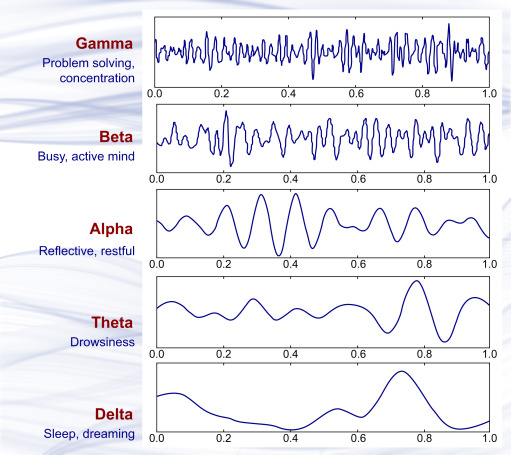
\includegraphics{images/Th-background/brainwaves.jpg}
    \caption{Brain wave samples with dominant frequencies belonging to beta, alpha, theta, and delta bands and gamma waves and their interpretations \cite{abhang_chapter_2016}}
    \label{fig:brainwaves}
\end{figure}

This signal-based analysis of different states helps medical researchers to gain a better understanding of the functional and behavioral characteristics of the complex structure of the brain.

\begin{figure}[ht]
    \centering
    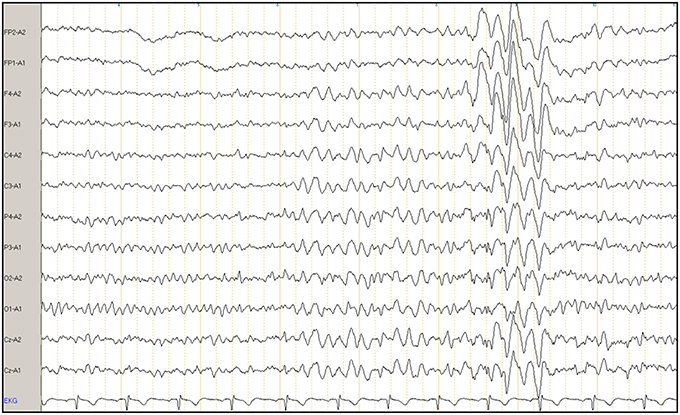
\includegraphics[width=1.0\textwidth]{images/Th-background/simple-eeg-trace.png}
    \caption{An \gls{EEG} trace \cite{tebartz_van_elst_increased_2016}}
    \label{fig:simple-eeg-trace}
\end{figure}

\subsection{Electrodes}
As stated above, \gls{EEG} is a commonly used non-invasive method for evaluating and monitoring brain activity \cite{hajare_comparative_2021}. It involves the placement of conductive electrodes on the scalp, which measure the potential difference created by the firing of neurons in the brain. In the traditional approach, several electrodes are placed at standard positions on the scalp. The voltage fluctuations, which are in the order of microvolts, are then amplified several thousand times.

EEG electrodes are made of conductive materials that measure the electrical potential difference between the bioelectric field from the scalp and its reference point. This voltage can only be detected on the scalp when a large number of neurons fire simultaneously. The collective activation of neurons in a neural mass, which consists of $10^4$ to $10^7$ neurons, is called synchronism \cite{bastos-filho_introduction_2020}. The result of these groups of cells being excited multiple times in a coordinated manner is a large number of rhythmic waves as the output. The sensors measure signals that originate from the brain, which vary over time \cite{hajare_comparative_2021}.

The accuracy of the measurement relies on the establishment of a low-resistance contact between the sensor and the scalp \cite{sullivan_low-noise_2007}. 
Gels are often used as a medium between the sensor and the patient's scalp to facilitate this contact. However, applying the gel can be time-consuming and may spread through the subject's hair, leading to shorting of the electrodes. The gel can also dry over time and be uncomfortable or irritating for the subject, potentially causing allergic reactions. In addition, the characteristics of the gel may change over time.

For these reasons other types of sensors have been proposed, such as dry metal and capacitive electrodes, the benefits of wet electrodes, particularly their low impedance and high sensitivity, make them the preferred choice for many electrophysiological applications.

\begin{figure}[ht]
    \centering
    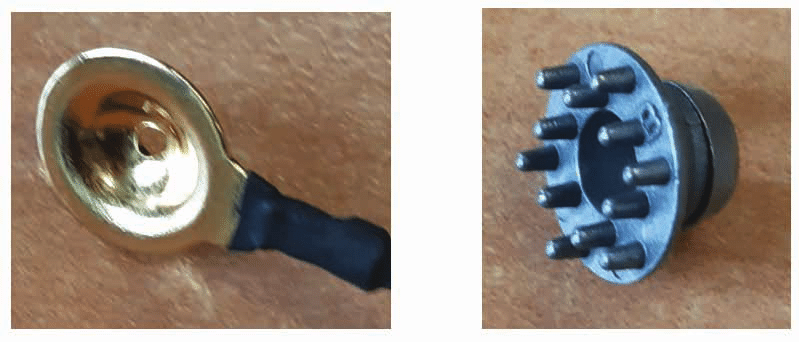
\includegraphics[width=1.0\textwidth]{images/Th-background/wet-dry-electrode.png}
    \caption{Standard EEG electrodes; gold cup wet electrode (left); and pin-shaped dry Ag/AgCl electrode (right) \cite{tseghai_status_2020}}
    \label{fig:wet_dry_electrodes}
\end{figure}

\subsection{Invasive EEG}
\gls{EEG} involves the use of electrodes placed on the scalp to detect and record the brain's electrical activity, which can provide valuable information about brain function and dysfunction \cite{mercier_advances_2022}. While scalp \gls{EEG} is widely used and is generally considered to be safe and well-tolerated, there is also a more invasive version of \gls{EEG} called \gls{iEEG}.

Intracranial EEG involves the insertion of electrodes directly into the brain tissue, usually through small holes drilled in the skull. This technique allows for the more precise measurement of brain activity, as the electrodes are in closer proximity to the brain tissue. However, the use of \gls{iEEG} is associated with a number of significant risks and drawbacks.

One major disadvantage of \gls{iEEG} is that it requires surgery to implant the electrodes, which can be risky and involves a significant recovery period. Additionally, the presence of electrodes within the brain tissue can alter brain function, making it difficult to interpret the recorded brain activity.

Given these risks and drawbacks, \gls{iEEG} is generally not used for routine epilepsy seizure prediction. While it may have some value in certain research or clinical contexts, the risks and invasiveness of the procedure make it unsuitable for widespread use in the management of epilepsy. Scalp EEG, on the other hand, is a safe and non-invasive alternative that is more commonly used for epilepsy seizure prediction.

\begin{figure}[ht]
    \centering
    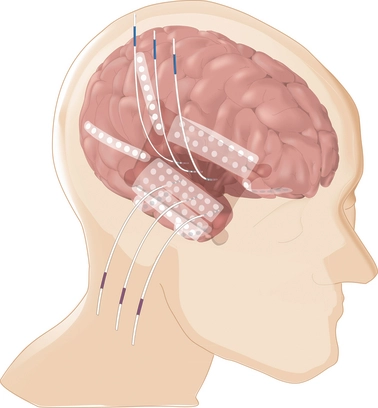
\includegraphics[scale=0.5]{images/Th-background/intracranialEEG.png}
    \caption{Schematic drawing of partial intracranial electrodes implantation for \gls{iEEG} \cite{surbeck_combination_2011}}
    \label{fig:intracranialEEG}
\end{figure}

\subsection{Standards for digital recording of clinical \glsentryshort{EEG}}
To ensure high-quality digital \gls{EEG} recording in clinical settings, standards have been established for recording, storing, reviewing, and exchanging \glspl{EEG} among clinicians and laboratories. These standards are specifically for digital EEG used in patient care. One particularly important standard is the 10-20 electrode placement protocol, which was adopted by the \gls{IFCN} \cite{nuwer_ifcn_1998}.

\subsubsection{The 10-20 electrode placement protocol}
This protocol standardizes the physical placements and designations of 21 electrodes on the scalp, using reference points on the skull to divide the head into proportional positions that adequately cover all brain regions \cite{rojas_study_2018}. Each electrode is named based on the region of the brain in which it is positioned (frontal, central, temporal, posterior, or occipital) and the cerebral hemisphere in which it is located (right or left).

\begin{figure}[ht]
    \centering
    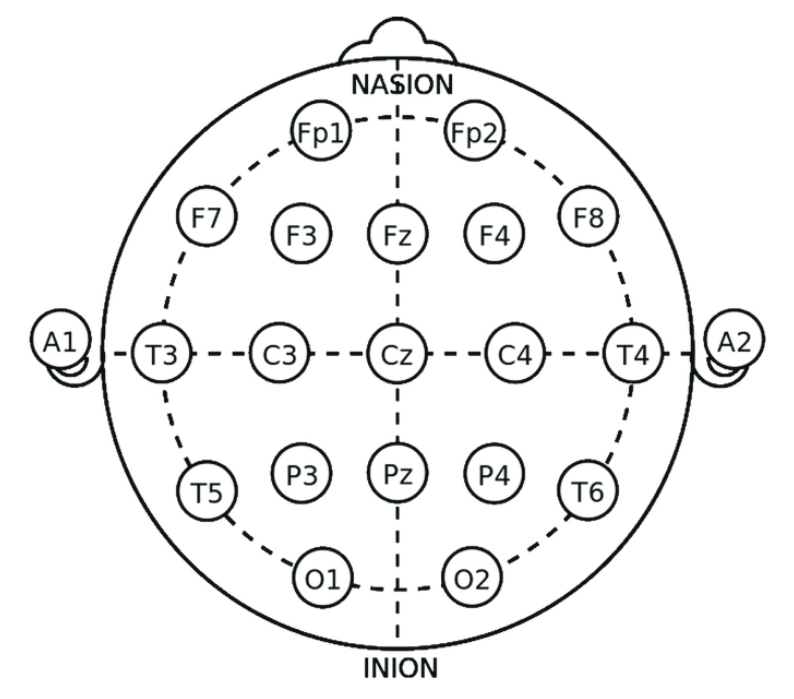
\includegraphics[width=0.5\textwidth]{images/Th-background/10-20-electrode-placement.png}
    \caption{The 10-20 International system of EEG electrode placement \cite{rojas_study_2018}}
    \label{fig:10-20-electrode-placement}
\end{figure}

The 10-20 system is commonly used in clinical settings, but there are also other standard placement protocols for EEG electrodes, such as the 10-10 system, which is more commonly used in research.

\subsubsection{\glsentrylong{EDF} (\glsentryshort{EDF})}
In order to facilitate the exchange and analysis of EEG data, various standards have also been adopted for storing and formatting EEG data. One such standard is the \gls{EDF} \cite{kemp_simple_1992}.

\gls{EDF} is a standard file format designed for the exchange and storage of medical time series data in general. 
It is an open and non-proprietary format that is commonly used to archive, exchange, and analyze data from commercial devices in a format that is independent of the acquisition system, allowing the data to be retrieved and analyzed by independent software. 
It was published in 1992 and stores multichannel data, allowing for different sample rates for each signal. It consists of a header and one or more data records, with the header containing general information (patient identification, start time) and technical specifications for each signal (calibration, sampling rate, filtering) encoded as ASCII characters, and the data records containing samples as little-endian 16-bit integers. 

\gls{EDF+} was published in 2003 and is largely compatible with \gls{EDF}, with all existing \gls{EDF} viewers also able to display \gls{EDF+} signals \cite{kemp_european_2003}. However, \gls{EDF+} files also allow for the coding of discontinuous recordings, as well as annotations, stimuli, and events in UTF-8 format.

\subsection{Artifacts}
\gls{EEG} has high temporal resolution, which causes its signals to be prone to contamination by unwanted noise, resulting in various artifacts \cite{jiang_removal_2019, raduntz_automated_2017}. 
Artifacts in \gls{EEG} data can be caused by environmental noise, experimental error, and physiological factors. Those that originate from external factors, such as environmental noise and experimental error, are classified as extrinsic artifacts, while those that come from the body itself, such as eye blinks, muscle activity, and heartbeats, are classified as intrinsic artifacts. 

These artifacts can interfere with neural information and even be mistaken as normal phenomena, potentially misleading practical applications such as brain-computer interfaces. In addition, artifacts may mimic cognitive or pathological activity, potentially biasing the visual interpretation and diagnosis in clinical research, such as in the analysis of sleep disorders or Alzheimer's disease. As a result, the identification and removal of artifacts is an important preprocessing step before the use of \gls{EEG} data in clinical diagnosis or practical applications.

The major physiological artifacts that can impact \gls{EEG} data will be discussed next.

\subsubsection{Ocular Artifacts}
Ocular artifacts, caused by eye movement and blinks, are a significant source of contamination in \gls{EEG} recordings \cite{wallstrom_automatic_2004}. These artifacts are recorded by \gls{EEG} activity due to changes in the orientation of the retina and cornea dipole or the contact of the cornea with the eyelid, and can also be recorded using \gls{EOG}. However, both \gls{EOG} and \gls{EEG} can contaminate each other, making it difficult to remove \gls{EOG} artifacts without introducing errors. 

\subsubsection{Muscle Artifacts}
Muscle activity, recorded by \gls{EMG}, is another difficult problem in \gls{EEG} data due to the wide range of frequencies (0 Hz to >200 Hz) at which it can occur and the difficulty in obtaining activity from single channel measurements \cite{goncharova_emg_2003}.

\subsubsection{Cardiac Artifacts}
Cardiac activity, including pulse artifacts caused by the expansion and contraction of blood vessels and \gls{ECG} signals from the electrical activity of the heart, can also contaminate \gls{EEG} data \cite{goncharova_emg_2003}.

\subsubsection{Extrinsic Artifacts}
External sources of artifacts, including instrument artifacts from electrode misplacement and cable movements and electromagnetic interference, can also affect \gls{EEG} recordings. These artifacts can be mitigated through appropriate procedures and filtering, but volume conduction artifacts, caused by the coherence between \gls{EEG} channels, can also be challenging to deal with \cite{sweeney_artifact_2012}.


\subsection{Applications}
\gls{EEG} is used to study the activity of the brain by recording postsynaptic potentials produced by neurons. This knowledge can be used to diagnose and detect brain disorders and related diseases, and to design better treatments. With the development of technology, the use of \gls{EEG} has also been expanded to other areas beyond just medical applications \cite{lai_literature_2018}.
These applications are medical, \gls{BCI} and neuromarketing. What follows is an overview of the possible applications of \gls{EEG} in these fields.

\subsubsection{Medical field}
\gls{EEG} has been extensively used to detect seizures and brain injuries, other than seizure prediction, which will be discussed later in more detail \cite{lai_literature_2018}. 
Various methods have been developed to extract features from \gls{EEG} signals for seizure detection, including wavelet domain analysis, parametric spectrum estimation techniques, and ictal rules on Poincare plane. Machine learning approaches, such as classifiers, are commonly used to discriminate normal and abnormal \gls{EEG} \cite{sharmila_epilepsy_2018}. 

For brain injury detection, animal brain models, classifiers, and techniques such as Fourier and wavelet transforms, power spectral density analysis, and evoked potentials are utilized. These approaches aim to identify quantitative \gls{EEG} features and generate activation maps to detect brain injury \cite{ianof_traumatic_2017, rapp_traumatic_2015}.


\subsubsection{ \glsentrylong{BCI} (\glsentryshort{BCI})}
\gls{BCI} is a way for humans to communicate with computers through their thoughts rather than physical movements \cite{lai_literature_2018}. This is made possible through the use of \gls{EEG}, which records brain activity and allows for explicit manipulation through thought. \gls{BCI} does not rely on the brain's normal pathways for communication through the peripheral nerves and muscles \cite{machado_eeg-based_2010}.

In object controlling applications, \glspl{BCI} that use \gls{EEG} have been used to control games, wheelchairs, and robot arms. In some cases, the \gls{BCI} requires the user to perform imagery movements in order to control the object, while in other cases it relies on \gls{EEG} features such as eye blinks \cite{huang_review_2021, liao_gaming_2012, al-qaysi_review_2018}.

In object recognition, \glspl{BCI} have been used to recognize imagery objects, taste, image familiarity, movement intention, attention stages, gaze, emotions, voice familiarity, and drowsiness. These applications often involve training a classifier on recorded \gls{EEG} data in order to classify the data into different categories \cite{mohedano_exploring_2015}.

In rehabilitation and human assistance, \glspl{BCI} have been used to aid patients with movement disorders, provide communication tools for nonverbal individuals, and assist with daily tasks such as controlling household appliances. Some examples of these applications include using \glspl{BCI} to control prostheses, enable individuals with severe motor impairments to communicate through spelling, and allow individuals to control appliances through imagery movements \cite{robinson_adaptive_2015}.

\subsubsection{ Neuromarketing }
Neuromarketing is a field that investigates how consumers respond to marketing stimuli using neuroscience techniques \cite{lai_literature_2018}. 
\gls{EEG} has commonly been used method in neuromarketing research due to its ease of setup and mobility. By analyzing \gls{EEG} recordings of subjects' brain activity while they are exposed to marketing stimuli, researchers can identify preferred marketing methods or products. There have been several studies in this area, including investigations into consumer preference for crackers, E-commerce products, automotive brands, tourist destinations, soap brands, bracelets, wine, and more. Some of these studies have employed deep learning techniques to classify preferences \cite{bazzani_is_2020, khurana_survey_2021}.


\section{Epileptic Seizures}
Epileptic seizures are episodes of abnormal brain activity that are characterized by sudden, involuntary changes in behavior, sensation, or consciousness. Seizures can vary in severity and duration, and they can be triggered by a variety of factors, including genetics, head injuries, and infectious diseases.

During a seizure, the brain's normal electrical activity becomes disrupted, and this can manifest in a variety of ways. Some people experience convulsions or muscle spasms, while others may experience changes in behavior or consciousness. Some seizures are mild and may only cause temporary confusion, while others can be more severe and result in loss of consciousness or injury.

In 2017, the \gls{ILAE} updated its classification system for different types of seizures \cite{fisher_instruction_2017, fisher_operational_2017}. This update was made to better reflect that some seizure types can have either a localized or generalized onset, to allow for classification when the onset is not witnessed, to include previously unclassified seizure types, and to use more straightforward names.

\subsection{Seizure types and classification}

According to the \gls{ILAE}, seizure classification begins by determining whether the initial manifestation of the seizure is focal (affecting a specific part of the brain) or generalized (affecting the entire brain) \cite{fisher_instruction_2017, fisher_operational_2017}. If the onset of the seizure is missed or not clear, the seizure is classified as unknown onset. Focal seizures are further subclassified based on the level of awareness the person experiences during the seizure and the presence of motor or nonmotor signs and symptoms at the onset. If the person is aware of themselves and their surroundings during the seizure, it is classified as a focal aware seizure. If the person experiences impaired awareness during any part of the seizure, it is classified as a focal impaired awareness seizure. Focal seizures can also be classified based on the dominant symptom or sign at the onset, such as a focal sensory seizure or a focal motor seizure. Seizure classification can stop at any level, depending on the available information and the purposes of the person classifying the seizure. It is also possible to classify a seizure based on both anatomic and behavioral features. In addition to these classifications, seizures can be described in free text to provide more detailed information about the features of the seizure. Such classification in summarized in Fig. \ref{fig:ILAE-seizure-types}.

As expected by this classification, during a focal seizure, the EEG may show abnormal activity in a specific area of the brain, while during a generalized seizure, the EEG may show abnormal activity across the entire brain, as shown in Fig. \ref{fig:eeg-seizure-partial-generalized}. These differences in EEG patterns can help to distinguish between the two types of seizures and inform treatment decisions \cite{raga_electroclinical_2021}.


\begin{figure}[t]
    \centering
    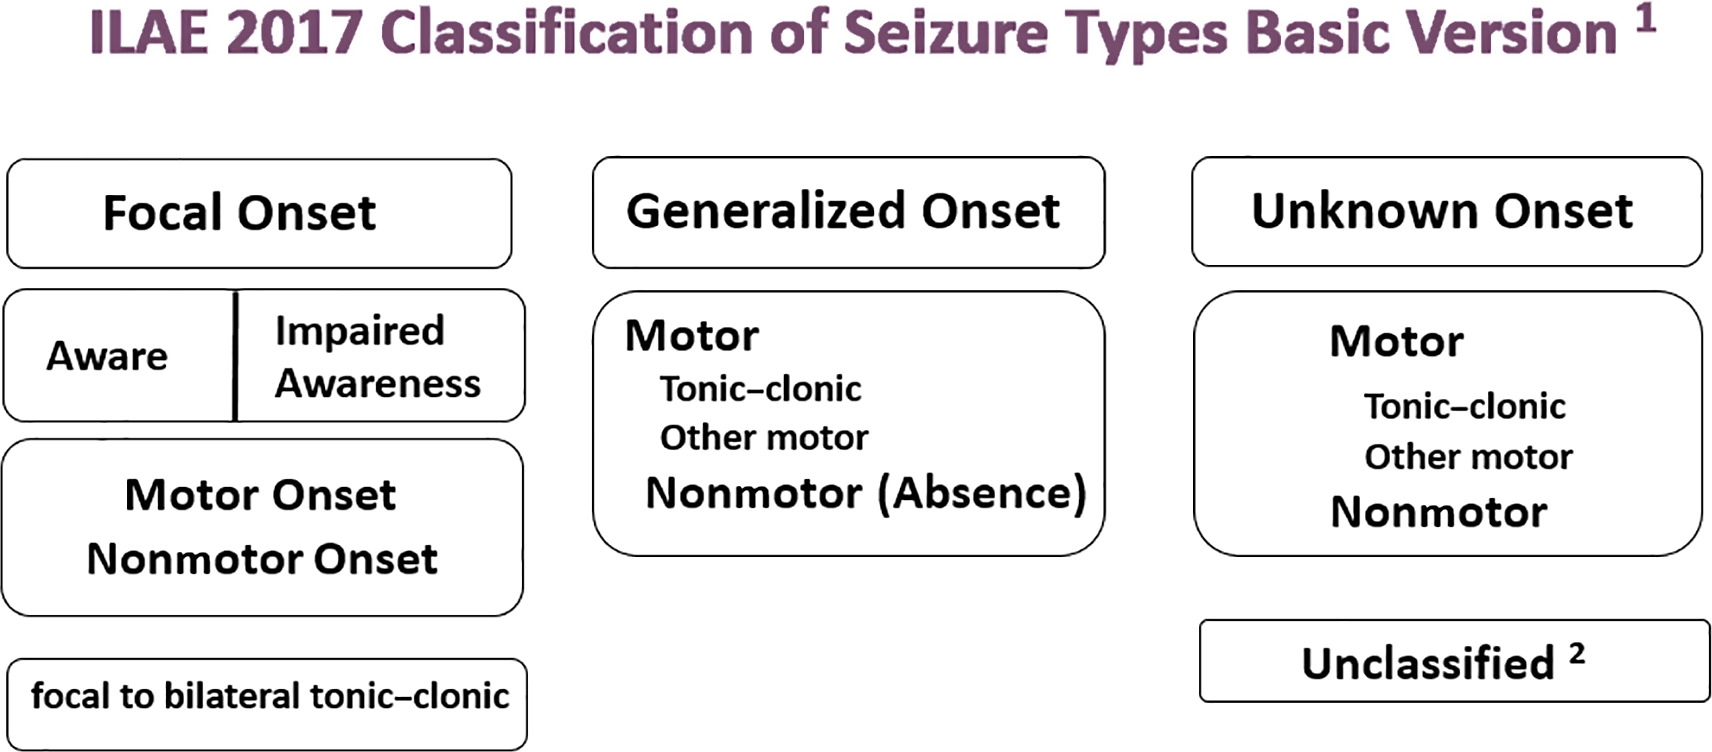
\includegraphics[width=0.75\textwidth]{images/Th-background/ILAE-seizure-types.png}
    \caption{The basic \glsentryshort{ILAE} 2017 operational classification of seizure types \cite{fisher_instruction_2017, fisher_operational_2017}}
    \label{fig:ILAE-seizure-types}
\end{figure}

\begin{figure}[t]
    \centering
    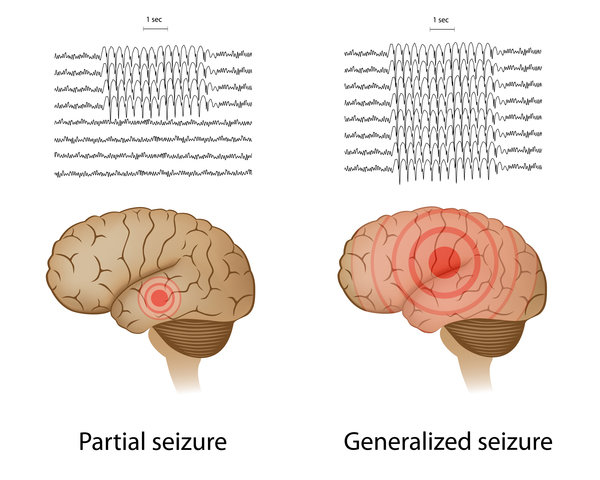
\includegraphics[width=1.0\textwidth]{images/Th-background/eeg-seizure-partial-generalized.jpg}
    \caption{Differences in EEG based on the type of seizure (focal on the left, generalized on the right)          \cite{bates_epileptic_2018}}
    \label{fig:eeg-seizure-partial-generalized}
\end{figure}

\subsection{\glsentryshort{EEG} phases w.r.t. epileptic seizures}
From the perspective of epileptogenesis \cite{aminoff_encyclopedia_2014} (the study of the development of epilepsy), seizures have a four-phase cycle consisting in the interictal, the preictal, the ictal and the postictal states \cite{cui_learning_2018, epilepsy_foundation_seizure_nodate, heidi_moawad_your_2020}, as shown in Fig. \ref{fig:seizure-phases}.

\begin{figure}[ht]
    \centering
    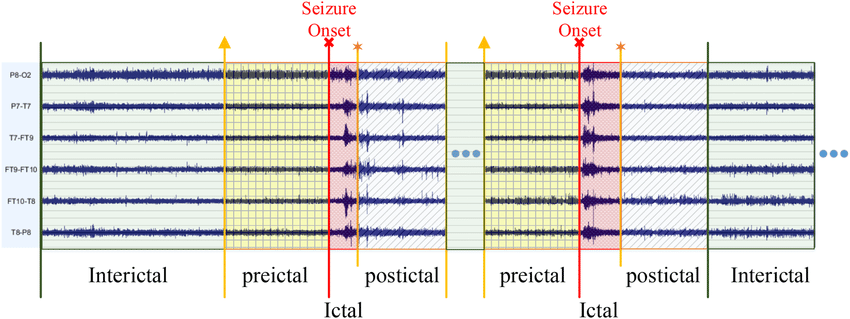
\includegraphics[width=1.0\textwidth]{images/Th-background/seizure-phases.png}
    \caption{Different phases of EEG signals w.r.t. epileptic seizures \cite{cui_learning_2018}}
    \label{fig:seizure-phases}
\end{figure}

The interictal phase is the period of time between seizures, during which a person is not experiencing any seizure activity. 

The preictal phase, also known as the aura phase, occurs just before a seizure and can vary in duration from person to person \cite{scaramelli_prodromal_2009}. 

The ictal phase is the actual seizure event, which can last for several seconds to several minutes. It is during this time that intense electrical activity is occurring in the brain. 

The postictal phase is the period after a seizure, during which a person is returning to their normal state of consciousness. This phase can last for several minutes to several hours and may be accompanied by confusion, fatigue, difficulty remembering the seizure, and physical symptoms such as headaches or muscle aches.

There is no established consensus on the duration of states other than the ictal state. 
For example, the postictal state can last for a few minutes, hours, or even days \cite{remi_clinical_2010}. Abnormalities associated with the preictal state can be observed for 30 to 90 minutes \cite{richardson_introductionepilepsy_2011}.

\section{Anomaly Detection}
Anomaly detection, also known as outlier detection or novelty detection, is the process of identifying data instances that deviate significantly from the majority of data instances \cite{pang_deep_2021}. The area has been actively researched for decades and is important in a variety of fields such as risk management, security, and medical care. In recent years, deep learning has shown great potential in learning complex data representations and has been used in developing deep anomaly detection methods, which have demonstrated potentially better performance than traditional methods.

Anomaly detection as a problem is strictly associated to unique complexities, specifically in the context of deep learning. These include the unknown nature of anomalies and the different characteristics they may have, the rarity of anomalous instances and the class imbalance this creates, and the variety of types of anomalies that can exist. Anomaly detection is a unique problem with many unknowns and characteristics that are different from majority of data instances, which makes it challenging for both deep and shallow detection methods. Furthermore, different types of anomaly such as point anomalies, conditional anomalies and group anomalies may require different methods to be detected properly \cite{chandola_anomaly_2009}.

\subsection{Supervision in Anomaly Detection Approaches}
There are three main approaches to anomaly detection, depending on the amount of anomalous data used during the training phase: fully supervised, semi-supervised, and unsupervised.
Each approach has its own advantages and limitations, therefore, the choice of the right approach depends on the problem and the availability of labeled data.

\subsubsection{Fully supervised}
Fully supervised anomaly detection requires labeled data, which includes both normal and anomalous examples. The model is trained using this labeled data and can then be used to identify anomalies in new, unlabeled data. The main advantage of fully supervised anomaly detection is that it can produce highly accurate results when enough labeled data is available. However, collecting labeled data for anomaly detection can be difficult and expensive, making fully supervised methods impractical in some cases.

\subsubsection{Semi-supervised}
Semi-supervised anomaly detection uses a set of labeled normal training data and some labeled anomaly data. The model is trained using the labeled normal data, and the labeled anomaly data is used to fine-tune the model and improve its ability to detect anomalies. This approach can be more practical than fully supervised methods as it does not require a large amount of labeled anomaly data.

\subsubsection{Unsupervised}
Unsupervised anomaly detection does not require any labeled data. Instead, the model is trained on the normal data and uses its understanding of the normal data distribution to identify unusual patterns in new, unlabeled data. The main advantage of unsupervised anomaly detection is that it does not require labeled data, which can be difficult to obtain. However, unsupervised methods can be less accurate than supervised methods, as they rely on assumptions about the distribution of anomalies.


\subsection{Challenges tackled by Deep Anomaly Detection}
The complexity of the problem of anomaly detection leads to various challenges. 
Some of these challenges, such as the ability to handle large amounts of data, have been successfully addressed in recent years. However, other challenges remain unresolved and deep anomaly detection may be able to make significant contributions to addressing them.

\subsubsection{Low anomaly detection recall rate}
Anomaly detection methods have a difficult time identifying all anomalies because they are rare and heterogeneous, which can lead to many normal instances being reported as anomalies and true yet sophisticated anomalies being missed. 
Despite many methods being introduced over the years, current state-of-the-art methods still incur high false positives on real-world datasets. The challenge of reducing false positives and enhancing detection recall rates is one of the most important and difficult to solve, particularly because of the significant expense of failing to spot anomalies.

\subsubsection{Anomaly detection in high-dimensional and/or not-independent data}
Anomalies can be difficult to detect in high-dimensional spaces because they may not have obvious abnormal characteristics. One solution is to perform anomaly detection in a lower-dimensional space that is created by a subset of original features or new features. However, this approach may not capture important feature interactions and couplings that are essential in high-dimensional data. Additionally, it can be challenging to ensure that the new feature space preserves the necessary information for accurate detection, and to detect anomalies in instances that are dependent on each other, such as through temporal, spatial, graph-based or other relationships.

\subsubsection{Data-efficient learning of normality/abnormality}
As previously stated, collecting large amounts of labeled data for anomaly detection is challenging and costly, making fully supervised methods, which require both normal and anomaly data, impractical. In recent years, research has focused on unsupervised methods that do not require labeled data. However, these methods can be limited by their assumptions about the distribution of anomalies. 
In practice, it can be easier to obtain labeled normal data and some labeled anomaly data. Utilizing this available labeled data to learn representations of normality and abnormality is crucial for accurate anomaly detection. Semi-supervised anomaly detection, which uses a set of labeled normal data, and weakly supervised anomaly detection, which uses some labels for anomaly classes but with limitations such as partial or inaccurate labels, are research areas that address this problem. The challenges in these methods include learning expressive representations with limited labeled anomaly data and creating detection models that can handle novel anomalies.

\subsubsection{Noise-resilient anomaly detection}
Many semi-supervised anomaly detection methods rely on the assumption that the labeled training data is clean, which can be problematic if there are instances that are mistakenly labeled as the opposite class. In such cases, unsupervised methods may be used instead, but this approach doesn't make use of the genuine labeled data. Additionally, there is often a large amount of unlabeled data that contains anomalies. Noise-resilient models can use this data to improve anomaly detection. The noise in this context can refer to both mislabeled data or unlabeled anomalies. The main challenge is that the amount of noise can vary greatly between datasets and the noisy instances may be irregularly distributed in the data space.

\subsubsection{Detection of complex anomalies}
The majority of existing anomaly detection methods are designed for point anomalies, which cannot be used for conditional or group anomalies as they have different characteristics. One of the main challenges is to develop methods that can detect these other types of anomalies. Additionally, current methods usually focus on detecting anomalies from a single data source, while many applications require the ability to detect anomalies across multiple, heterogeneous data sources, such as multidimensional data, graphs, images, text, and audio. One of the challenges here is that some anomalies can only be identified when considering two or more data sources.

\subsubsection{Anomaly explanation}
In safety-critical domains, using anomaly detection models as black-box models can lead to significant risks. For example, rare data instances reported as anomalies may result in algorithmic bias against minority groups, such as underrepresented groups in fraud or crime detection systems. To mitigate these risks, anomaly explanation algorithms that provide clear explanations for why a specific data instance is identified as an anomaly can be useful. These explanations can be reviewed by human experts to correct any bias. Providing explanations can be as important as detection accuracy in some applications. However, most anomaly detection studies focus on detection accuracy alone and do not consider the ability to provide explanations. Deriving anomaly explanations from specific detection methods is still an open problem, especially for complex models. Developing interpretable anomaly detection models that balance interpretability and effectiveness is also a major challenge.